\section{TANH Hyperbolic Tangent Function}

\subsection{Usage}

Computes the hyperbolic tangent of the argument.
The syntax for its use is
\begin{verbatim}
   y = tanh(x)
\end{verbatim}
\subsection{Function Internals}

The \verb|tanh| function is computed from the formula
\[
   \tanh(x) = \frac{\sinh(x)}{\cosh(x)}
\]
\subsection{Examples}

Here is a simple plot of the hyperbolic tangent function
\begin{verbatim}
--> x = linspace(-5,5);
--> plot(x,tanh(x)); grid('on');
\end{verbatim}


\centerline{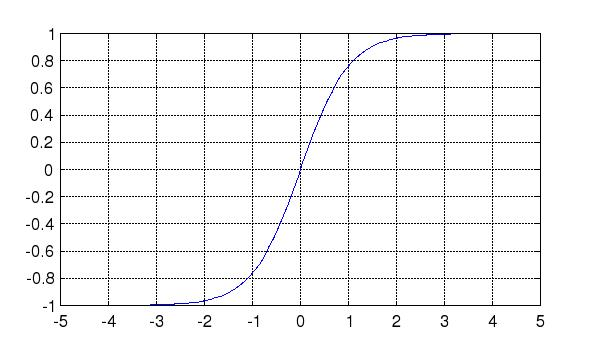
\includegraphics[width=8cm]{tanhplot}}

